% dqd_model_sketch.tex — the constant-capacitance model in the arrangement
% of your hand sketch: the sensor above, the two dots below, the plunger
% gates out to the sides.  All twelve couplings, and the matrices in full.
%
% A THIRD figure.  dqd_model.png and dqd_model_full.* both stay as they are.
%
% Differences from the sketch, and why:
%   * gate 3 is in.  The sketch has only Vg1 and Vg2, which leaves out
%     c_{d_1g_3}, c_{d_2g_3} and c_{s_1g_3}; the last of those is the
%     largest entry of C_sg.  It sits above the sensor, where its wire to
%     QD_s is short and meets nothing.
%   * the sensor keeps its index: c_{s_1g_1}, not c_{sg_1}, so a symbol in
%     the drawing is the same symbol as in the matrix.
%
% Three gates each coupling to three islands is K_{3,3}, which is not
% planar, so a crossing-free drawing does not exist.  This arrangement takes
% three crossings, each with the usual semicircular hop; the wide-arc
% version in dqd_model_full.tex takes one but spends a lot of paper on it.
%
% Build:
%     pdflatex dqd_model_sketch.tex
%
% THIS IS THE COLOURED TWIN of dqd_model_sketch.tex; that file is unchanged.
% Colour is applied to panel (a) only -- the matrices in (b) stay black,
% because a matrix entry is not a wire, and colouring one would claim a
% grouping the algebra does not have.
%
\documentclass[border=10pt]{standalone}
\usepackage{amsmath}
\usepackage{tikz}
\usetikzlibrary{calc,intersections}

% ── the palette ───────────────────────────────────────────────────────────
% Colour says what a coupling DOES.  Checked on white with the six-check
% validator: worst normal-vision dE 16.3, worst colour-vision-deficient dE
% 8.4 (target 8), every hue at or above 3.0 contrast.
\definecolor{cPrim}{HTML}{2A78D6}   % plunger gate -> its own dot: the period
\definecolor{cCross}{HTML}{EB6834}  % cross-coupling: the slope of the lines
\definecolor{cInter}{HTML}{4A3AA7}  % interdot: the anticrossing
\definecolor{cSens}{HTML}{199E70}   % the sensor's couplings: readout
\definecolor{cWeak}{HTML}{8A8F98}   % gate 3 to the dots: the smallest entries


\begin{document}
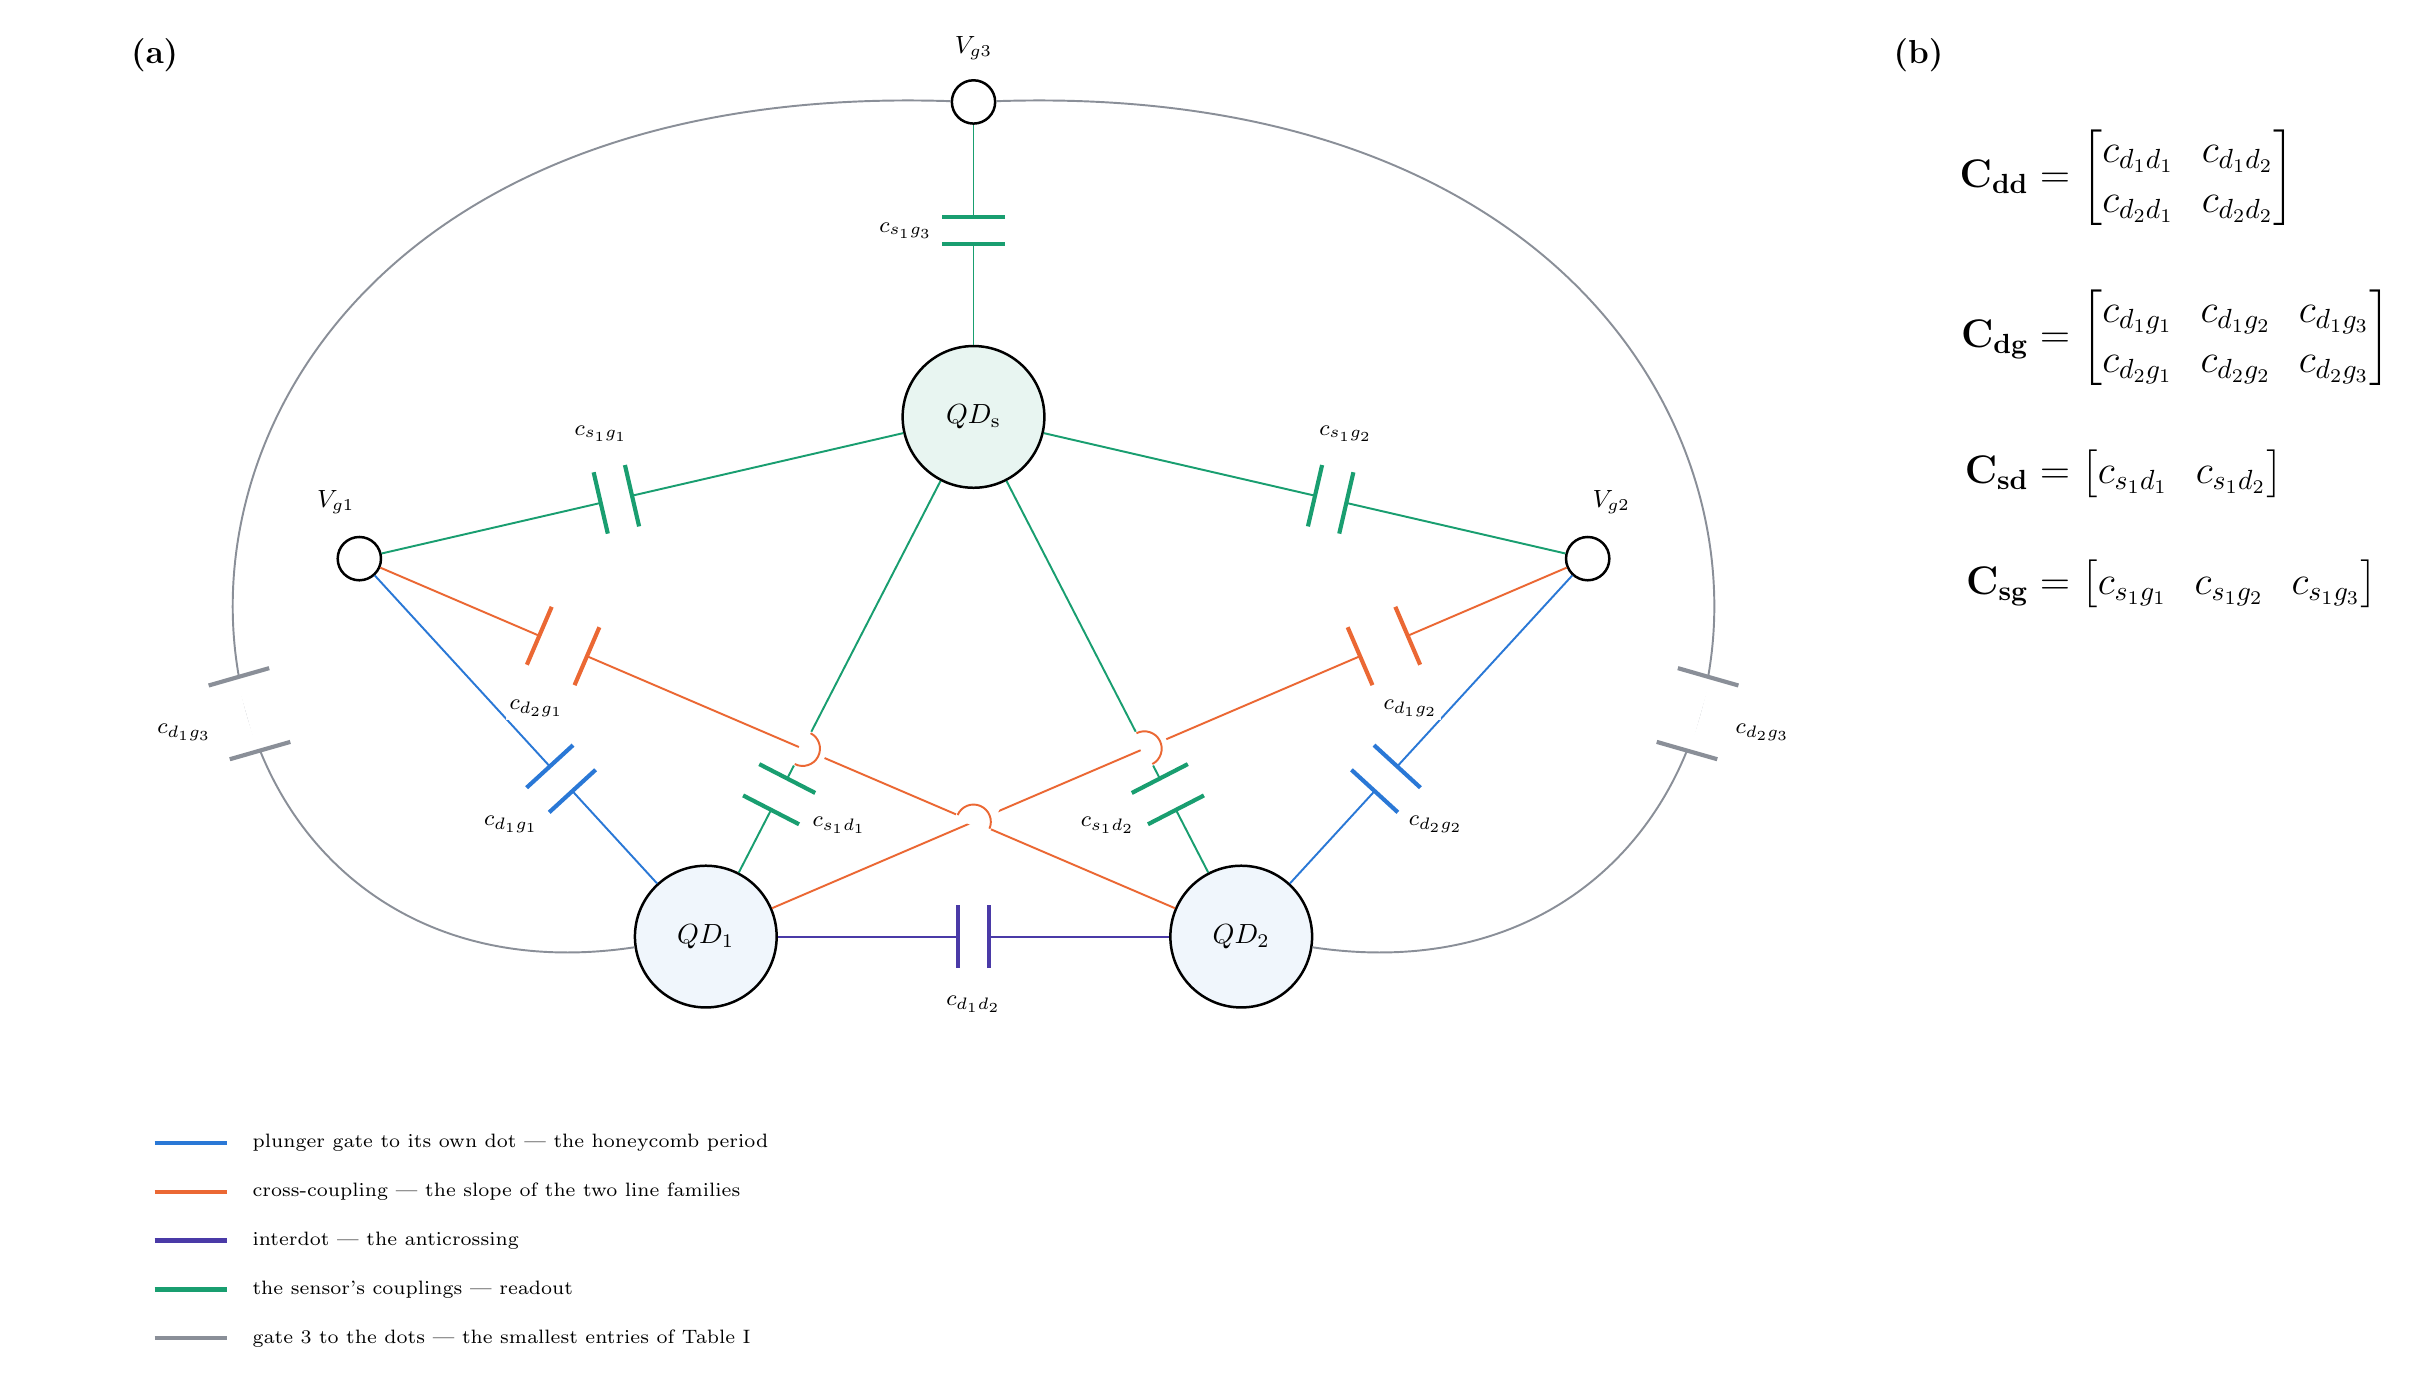
\begin{tikzpicture}[
    island/.style = {circle, draw, line width=0.9pt, minimum size=18mm,
                     fill=cPrim!7, inner sep=0pt},
    sensor/.style = {circle, draw, line width=0.9pt, minimum size=18mm,
                     fill=cSens!10, inner sep=0pt},
    gate/.style   = {circle, draw, line width=0.9pt, minimum size=5.5mm,
                     fill=white, inner sep=0pt},
    wire/.style   = {line width=0.7pt},
    lab/.style    = {font=\footnotesize, inner sep=1.4pt,
                     fill=white, fill opacity=0.92, text opacity=1},
  ]

  % ── nodes ──────────────────────────────────────────────────────────────
  \node[gate]   (g3) at ( 0.0,  8.4) {};
  \node[sensor] (s1) at ( 0.0,  4.4) {$QD_\mathrm{s}$};
  \node[gate]   (g1) at (-7.8,  2.6) {};
  \node[gate]   (g2) at ( 7.8,  2.6) {};
  \node[island] (d1) at (-3.4, -2.2) {$QD_1$};
  \node[island] (d2) at ( 3.4, -2.2) {$QD_2$};

  \node[font=\small] at ($(g3)+(0,0.68)$)   {$V_{g3}$};
  \node[font=\small] at ($(g1)+(-0.30,0.72)$) {$V_{g1}$};
  \node[font=\small] at ($(g2)+( 0.30,0.72)$) {$V_{g2}$};

  % ── the capacitor symbol ───────────────────────────────────────────────
  % #1,#2  two points a short way apart on the wire; the plates are drawn
  %        square to the line joining them, so this works on a curve too.
  % #3     label, #4 the side (90 or -90) it is pushed to
  \def\platecolour{black}
  \newcommand{\plates}[4]{%
    \draw[white, line width=2.2pt] (#1) -- (#2);
    \draw[line width=1.5pt, \platecolour] ($(#1)!0.40cm!90:(#2)$) --
                            ($(#1)!0.40cm!-90:(#2)$);
    \draw[line width=1.5pt, \platecolour] ($(#2)!0.40cm!90:(#1)$) --
                            ($(#2)!0.40cm!-90:(#1)$);
    \node[lab] at ($($(#1)!0.5!(#2)$)!0.86cm!#4:(#2)$) {$c_{#3}$};
  }

  % a hop where two wires cross: #1 the point, #2--#3 the direction of the
  % wire that goes over
  \newcommand{\hop}[3]{%
    \pgfmathanglebetweenpoints{\pgfpointanchor{#2}{center}}%
                              {\pgfpointanchor{#3}{center}}%
    \edef\hopangle{\pgfmathresult}%
    \begin{scope}[shift={(#1)}, rotate=\hopangle]
      \fill[white] (-0.24,-0.05) rectangle (0.24,0.30);
      \draw[wire, cCross] (-0.22,0) arc (180:0:0.22);
    \end{scope}
  }

  % ── wires ──────────────────────────────────────────────────────────────
  \draw[wire, cSens] (g1) -- (s1);
  \draw[wire, cSens] (g2) -- (s1);
  \draw[wire, cSens, name path=sd1] (s1) -- (d1);
  \draw[wire, cSens, name path=sd2] (s1) -- (d2);
  \draw[wire, cPrim] (g1) -- (d1);
  \draw[wire, cPrim] (g2) -- (d2);
  \draw[wire, cCross, name path=x1] (g1) -- (d2);
  \draw[wire, cCross, name path=x2] (g2) -- (d1);
  \draw[wire, cInter] (d1) -- (d2);
  \draw[wire, cSens] (g3) -- (s1);
  \draw[wire, cWeak] (g3) .. controls (-12.0,8.8) and (-11.4,-3.4) .. (d1);
  \draw[wire, cWeak] (g3) .. controls ( 12.0,8.8) and ( 11.4,-3.4) .. (d2);

  % ── the three crossings ────────────────────────────────────────────────
  \path[name intersections={of=x1 and x2,  by=c0}];
  \path[name intersections={of=x1 and sd1, by=c1}];
  \path[name intersections={of=x2 and sd2, by=c2}];
  \hop{c0}{g1}{d2}
  \hop{c1}{s1}{d1}
  \hop{c2}{s1}{d2}

  % ── the plates ─────────────────────────────────────────────────────────
  \path (g1) -- (s1) coordinate[pos=0.42] (a1) coordinate[pos=0.48] (a2);
  {\def\platecolour{cSens}\plates{a1}{a2}{s_1g_1}{90}}
  \path (g2) -- (s1) coordinate[pos=0.42] (b1) coordinate[pos=0.48] (b2);
  {\def\platecolour{cSens}\plates{b1}{b2}{s_1g_2}{-90}}

  \path (s1) -- (d1) coordinate[pos=0.76] (c3) coordinate[pos=0.84] (c4);
  {\def\platecolour{cSens}\plates{c3}{c4}{s_1d_1}{90}}
  \path (s1) -- (d2) coordinate[pos=0.76] (d3) coordinate[pos=0.84] (d4);
  {\def\platecolour{cSens}\plates{d3}{d4}{s_1d_2}{-90}}

  \path (g1) -- (d1) coordinate[pos=0.62] (e1) coordinate[pos=0.70] (e2);
  {\def\platecolour{cPrim}\plates{e1}{e2}{d_1g_1}{-90}}
  \path (g2) -- (d2) coordinate[pos=0.62] (f1) coordinate[pos=0.70] (f2);
  {\def\platecolour{cPrim}\plates{f1}{f2}{d_2g_2}{90}}

  \path (g1) -- (d2) coordinate[pos=0.20] (h1) coordinate[pos=0.26] (h2);
  {\def\platecolour{cCross}\plates{h1}{h2}{d_2g_1}{-90}}
  \path (g2) -- (d1) coordinate[pos=0.20] (i1) coordinate[pos=0.26] (i2);
  {\def\platecolour{cCross}\plates{i1}{i2}{d_1g_2}{90}}

  \path (d1) -- (d2) coordinate[pos=0.46] (j1) coordinate[pos=0.54] (j2);
  {\def\platecolour{cInter}\plates{j1}{j2}{d_1d_2}{-90}}
  \path (g3) -- (s1) coordinate[pos=0.42] (k1) coordinate[pos=0.54] (k2);
  {\def\platecolour{cSens}\plates{k1}{k2}{s_1g_3}{-90}}

  \path (g3) .. controls (-12.0,8.8) and (-11.4,-3.4) .. (d1)
        coordinate[pos=0.60] (l1) coordinate[pos=0.66] (l2);
  {\def\platecolour{cWeak}\plates{l1}{l2}{d_1g_3}{-90}}
  \path (g3) .. controls (12.0,8.8) and (11.4,-3.4) .. (d2)
        coordinate[pos=0.60] (m1) coordinate[pos=0.66] (m2);
  {\def\platecolour{cWeak}\plates{m1}{m2}{d_2g_3}{90}}

  \node[font=\bfseries\large] at (-10.4, 9.0) {(a)};

  % ── (b) the matrices, in full ──────────────────────────────────────────
  \node[anchor=north west, font=\Large] at (12.4, 8.2) {$\begin{aligned}
      \mathbf{C}_{\mathbf{dd}} &=
        \begin{bmatrix}
          c_{d_1 d_1} & c_{d_1 d_2} \\
          c_{d_2 d_1} & c_{d_2 d_2}
        \end{bmatrix} \\[18pt]
      \mathbf{C}_{\mathbf{dg}} &=
        \begin{bmatrix}
          c_{d_1 g_1} & c_{d_1 g_2} & c_{d_1 g_3} \\
          c_{d_2 g_1} & c_{d_2 g_2} & c_{d_2 g_3}
        \end{bmatrix} \\[18pt]
      \mathbf{C}_{\mathbf{sd}} &=
        \begin{bmatrix}
          c_{s_1 d_1} & c_{s_1 d_2}
        \end{bmatrix} \\[18pt]
      \mathbf{C}_{\mathbf{sg}} &=
        \begin{bmatrix}
          c_{s_1 g_1} & c_{s_1 g_2} & c_{s_1 g_3}
        \end{bmatrix}
    \end{aligned}$};
  \node[font=\bfseries\large] at (12.0, 9.0) {(b)};


  % ── the key ────────────────────────────────────────────────────────────
  % Identity is never colour alone: every wire carries its own label as well.
  \begin{scope}[shift={(-10.4,-4.2)}]
    \foreach \col/\txt [count=\i] in {%%
        cPrim/{plunger gate to its own dot \textemdash\ the honeycomb period},
        cCross/{cross-coupling \textemdash\ the slope of the two line families},
        cInter/{interdot \textemdash\ the anticrossing},
        cSens/{the sensor's couplings \textemdash\ readout},
        cWeak/{gate 3 to the dots \textemdash\ the smallest entries of Table I}}
      {
        \draw[\col, line width=1.6pt]
          (0, -0.62*\i) -- ++(0.92,0);
        \node[anchor=west, font=\scriptsize, text=black]
          at (1.12, -0.62*\i) {\txt};
      }
  \end{scope}

\end{tikzpicture}
\end{document}
